% HET IP section

%----------------------------------------------------------------
% Demonstration of convolution to fit iodine atlas
% plot made by ~/Exo.../HET.../plots_general/convol_kernel/deconv_plot.pro
\begin{figure}
\centering
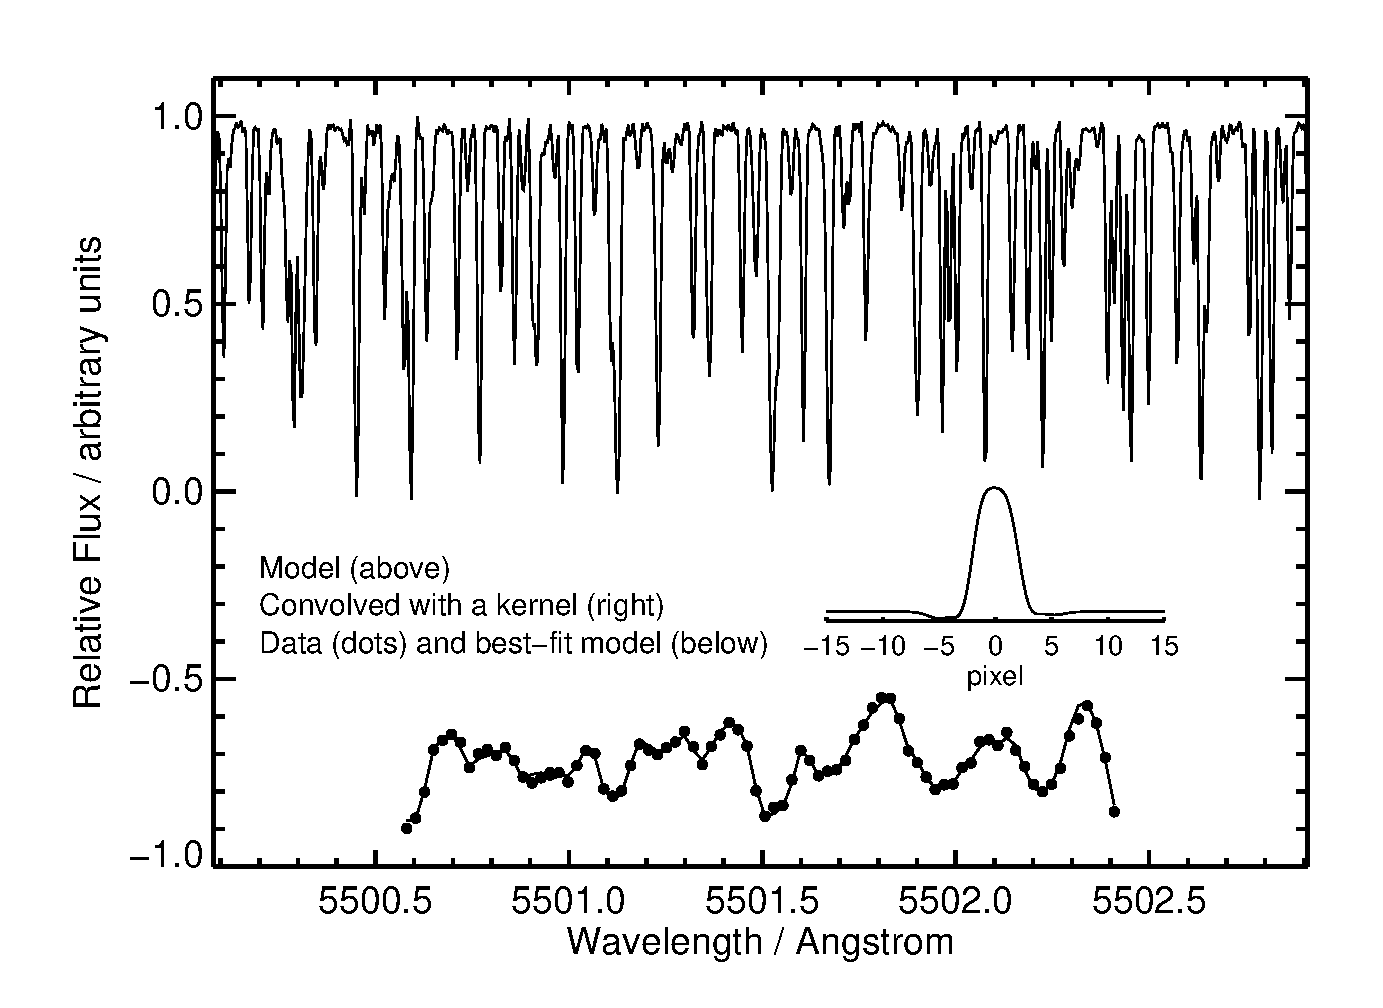
\includegraphics[scale=0.45]{het/convolution_kernel.eps}
\caption{Illustration of convolving the iodine atlas (sharp solid
  lines) with a kernel (middle right insert) to fit the observed
  iodine lines (black dots near the bottom, with best-fit model
  plotted in solid line).
\label{het:fig:convkernel}}
\end{figure}
%----------------------------------------------------------------





%----------------------------------------------------------------
% Comparison between HET and Keck chunk fit
% plot made by ~/Exo.../HET.../plots_general/fit_demo/plotfit.pro
\begin{figure}
\centering
\subfloat[\het\ Chunk]{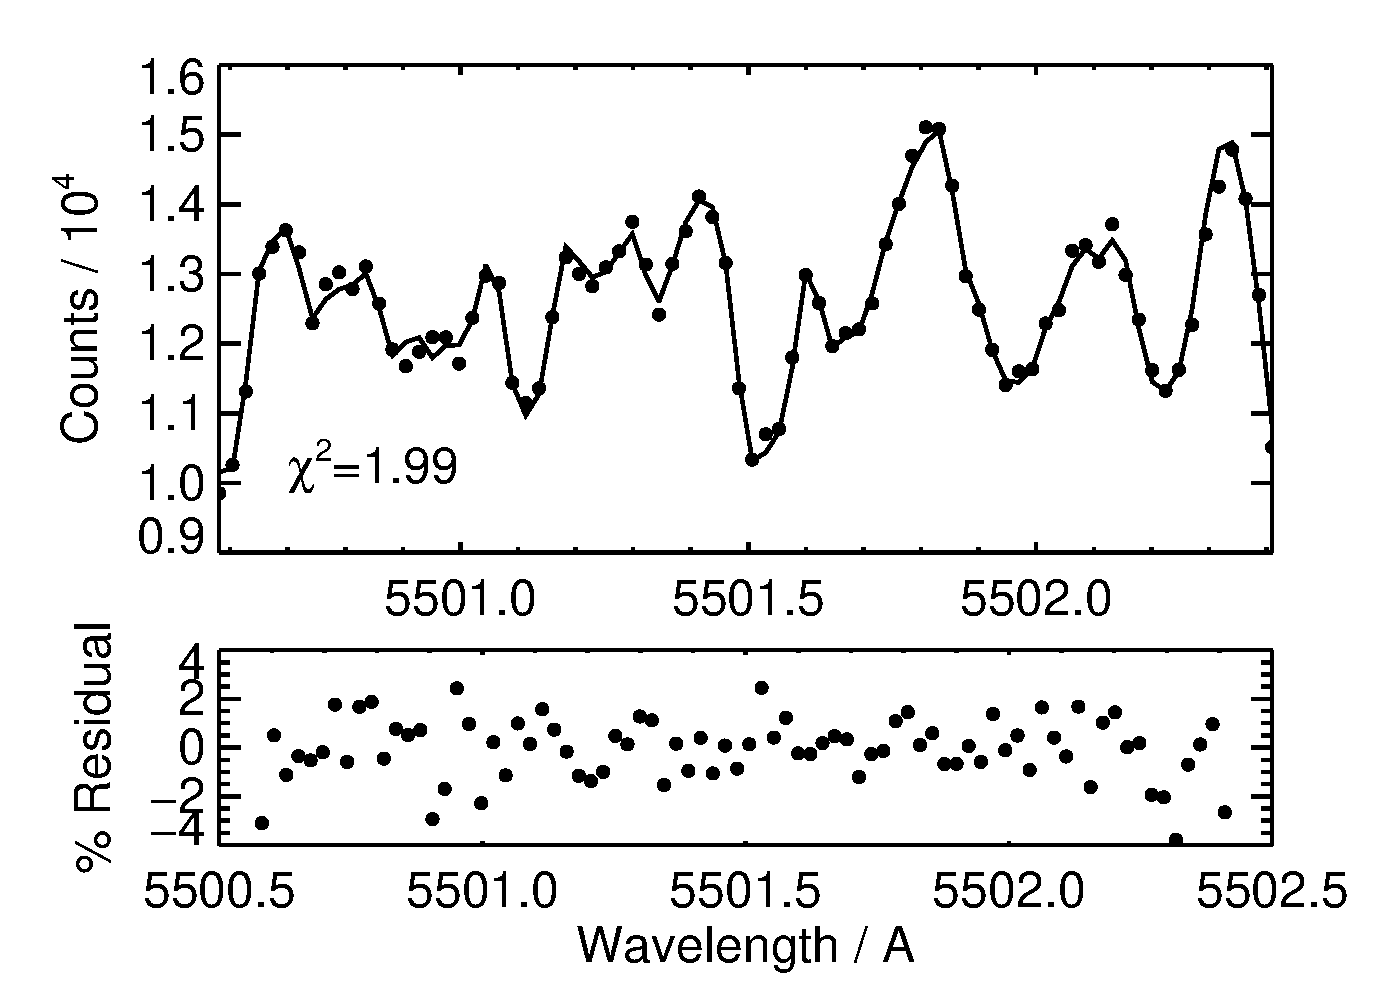
\includegraphics[scale=0.35]{het/20120124.176005.chunk189.eps}}
\subfloat[\keck\ Chunk]{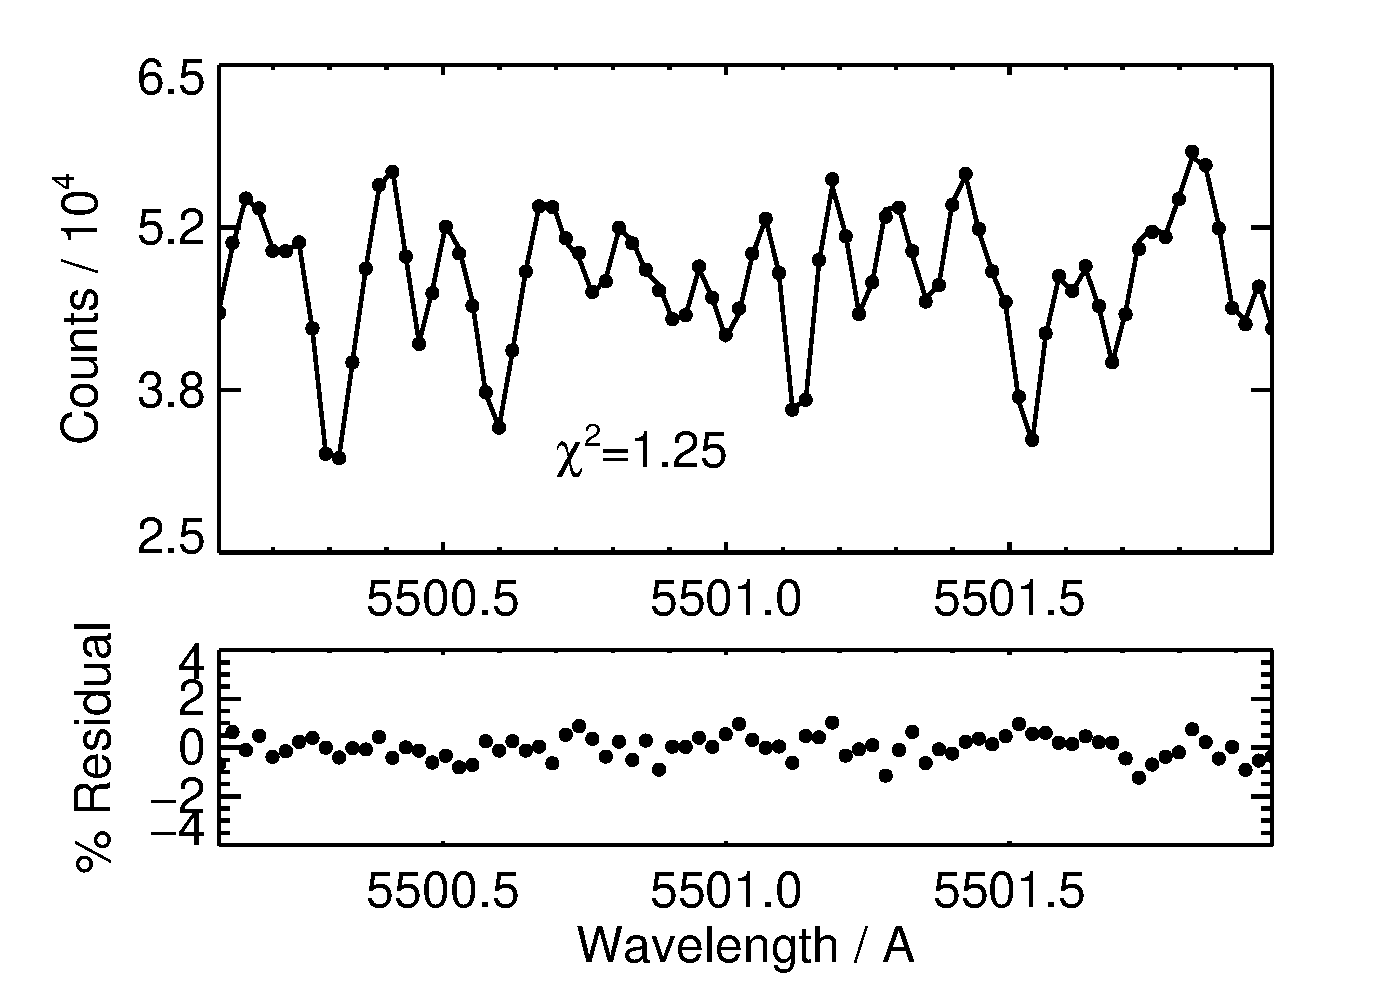
\includegraphics[scale=0.35]{het/rj82.77.chunk308.eps}}
\caption{Comparison between fits for a typical iodine-only chunk using
  \het\ data (left panel) and \keck\ data (right panel). Bottom panels
  are showing the residuals against best-fit models, plotted on the
  same $y$-axis scale. \het\ fit is significantly worse than \keck,
  which we believe is one of the major drivers behind \het's poorer RV
  precision. 
\label{het:fig:iodchunkcomp}}
\end{figure}
%----------------------------------------------------------------






%----------------------------------------------------------------
% Comparing 2005 and 2008 data, with GH and Gaussian IPs
% plot from ~/ExoPlanet-2010-2011/Professional_Development/201000-NSF_Jason/plots/
\begin{figure}
\centering
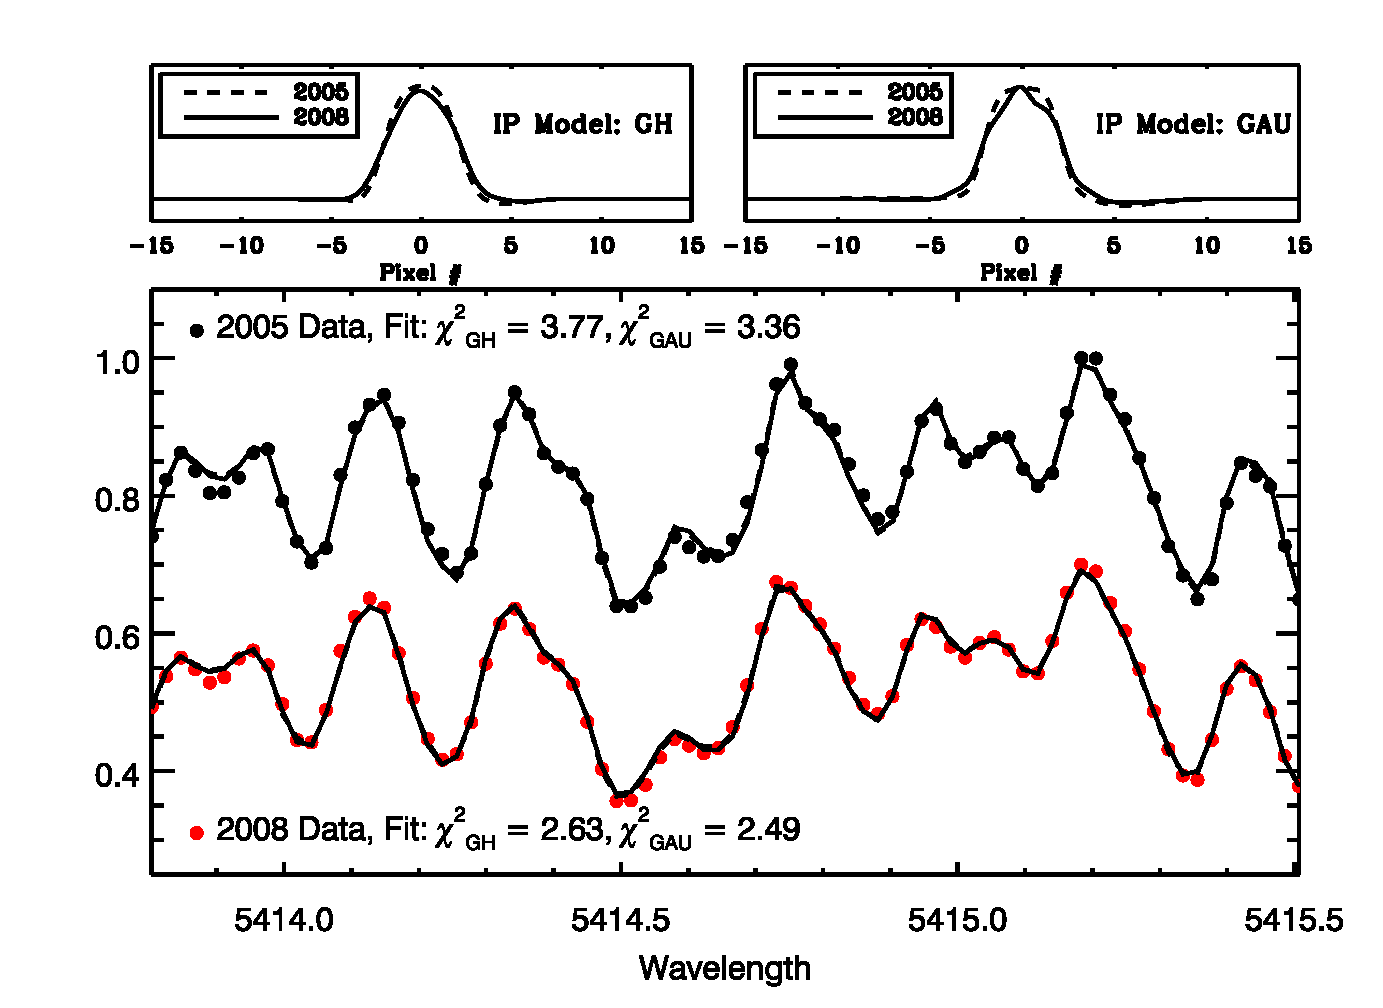
\includegraphics[scale=0.45]{het/iodfit.eps}
\caption{Illustration of fitting the iodine-only data (bottom panel)
  using different IPs (top panels), in this case, using GH and sum of
  Gaussians (GAU). These two IPs are practically ``equally bad",
  having similarly large reduced $\chi^2$ but neither produces a
  satisfactory fit. It is also interesting to see how ``stable" the
  best-fit IP can be across the years (i.e., in 2005 vs.~2008),
  hinting that the best IP may take a simple, smooth, and
  slowly-varying form. 
\label{het:fig:ghgau}}
\end{figure}
%----------------------------------------------------------------




%----------------------------------------------------------------
% Comparing Keck and HET IPs in Fourier space
% plot from screen shot of a slide in
% ~/ExoPlanet-2010-2011/Professional_Development/20150727-ThesisCommMeet/
% original plot is from ~/Exo../HET.../06-line.../powspec.pro and stored in ./plots/
\begin{figure}
\centering
\includegraphics[scale=0.45]{het/fftip.eps}
\caption{Fourier transform or power spectrum of a \het\ iodine-only
  spectrum (black dots) and its smoothed version (blue line). There is
  a clear signature of the \het\ slit at 4.3 pixel (corresponding to
  slit width for resolution R $=$ 60k). For comparison, the red curve
  is for \keck\ data, which shows no clear signiture of a slit,
  because \keck\ is not fiber-fed and the PSF of the star falls mostly
  within its slit.
\label{het:fig:fftip}}
\end{figure}
%----------------------------------------------------------------


One limiting factor for the current RV precision of \hrs\ is the
modeling of its instrumental profile (IP, or the spectrograph response
function or spectral PSF). In our original proposal, we promised to
look for a better IP for \hrs, as a test case for future fiber-fed
precise RV spectrographs, such as the upcoming MINERVA and the future
fiber-fed Keck/HIRES.

The old IP model for \hrs\ is the very versatile, orthogonal,
11-parameter Gauss-Hermite polynomials (GH). However, through our
analyses using calibration frames in Fourier space, we have found that
although GH is probably sufficient to describe the \hrs\ IP, because
of its ultra flexibility and multi-parameters, it deeply complicates
the $\chi^2$ space and very often hinders the fitter from finding the
true minimal (to address the issue with the fitter, see next section
and future plans). A simpler IP is therefore in great desire.

We have found a better IP function for \hrs, the modified Moffat function:
\begin{equation}
[1+(x/\theta)^2]^{-\beta\cdot(x/\delta)^2}
\end{equation} 
It is called the ``modified" Moffat function because the original
Moffat function does not have the $(x/\delta)^2$ term. We added this
term to add flexibility at the wings to enable change of characteristic
IP width while preserving wing profile. Figure~\ref{fig:ip}
illustrates the results: black line is the $\chi^2_\nu$ distribution
for fitting spectral chunks in an observation with GH IP; red line is
for modified Moffat IP; and dashed red is for fixing the IP in the
shape of a thorium line (proving that thorium line is a good proxy for
IP). This 3-parameter function fits the \hrs\ data almost equally
well, and it fits very well to the observed thorium line
(Figure~\ref{fig:ip} inset, dots are observed thorium line).

This modified Moffat function is potentially applicable to other
fiber-fed instruments, since these instruments tend to have IPs with
the same characteristic flat top and sharp wings.

Our ongoing work includes: adding small perturbation terms to the
modified Moffat IP to account for IP asymmetry and subtle wings due to
scattered light etc.; disentangling the effects of a bad IP model and
bad iodine atlas (as described in previous section); and other tests
with the aim to bring $\chi^2_\nu$ for fitting \hrs\ data to $\sim 1$,
which is what is achieved at Keck and enabled $\sim 1$ \mps\ RV
precision.





%----------------------------------------------------------------
% Comparing fits with two IPs
% plot made by ~/Exo.../HET.../plots_general/fit_demo/compfit.pro
\begin{figure}
\centering
\subfloat{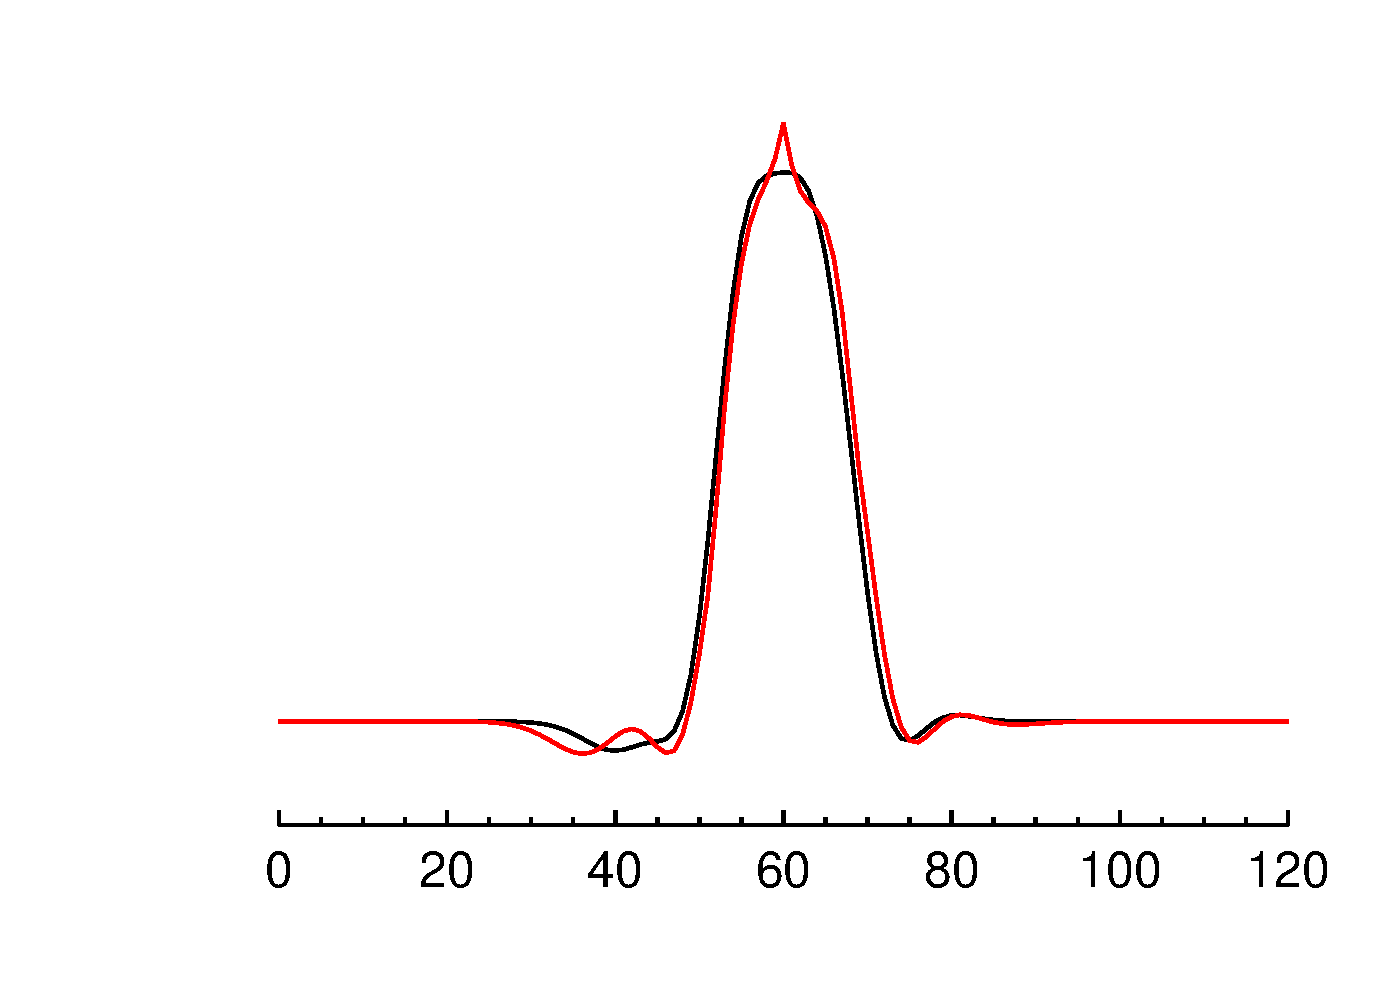
\includegraphics[scale=0.3]{het/20120124.176005.chunk191.compip.eps}}
\subfloat{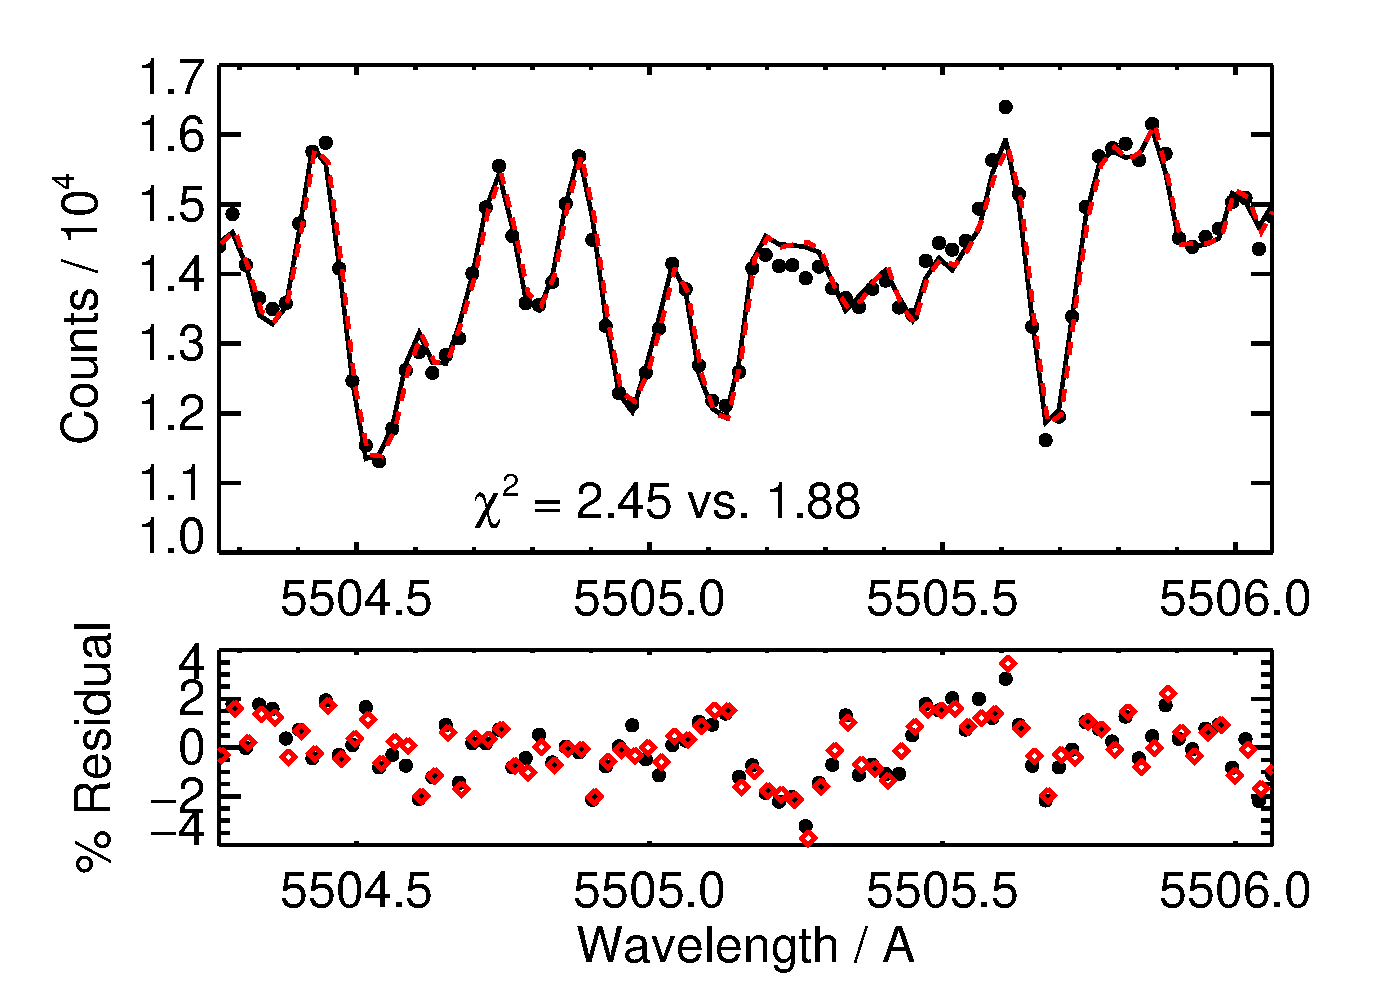
\includegraphics[scale=0.35]{het/20120124.176005.chunk191.compfit.eps}}
\caption{Introducing a sharp feature into the \het\ IP model, a
  triangle on top of the GH IP (red curve in the left panel), produces
  a better fit, somewhat to our surprise. The black in the left panel
  is the best-fit GH IP. GH$+$triangle is the IP model that produces
  the least $\chi^2_\nu$ among all of our IP models. However, as shown
  by the right panel, the two fits barely have any visible difference
  (red curve for GH$+$triangle IP and black for GH; bottom panel plots
  the residuals). Such a sharp feature in the IP is unphysical, and we
  interpretate this results as a hint for an unreliable iodine atlas
  (the sharp peak at the center is perhaps the IP model trying to
  ``stretch" the iodine lines deeper; see Section~\ref{het:sec:fts}
  for more details).
\label{het:fig:iodipcomp}}
\end{figure}
%----------------------------------------------------------------




%----------------------------------------------------------------
% Fitting with a Moffat function
% plot made by ~/ExoPlanet-2010-2011/HET-HRS-IP/06-line_through_dots/thar.pro
% and stored in ./plots/
\begin{figure}
\centering
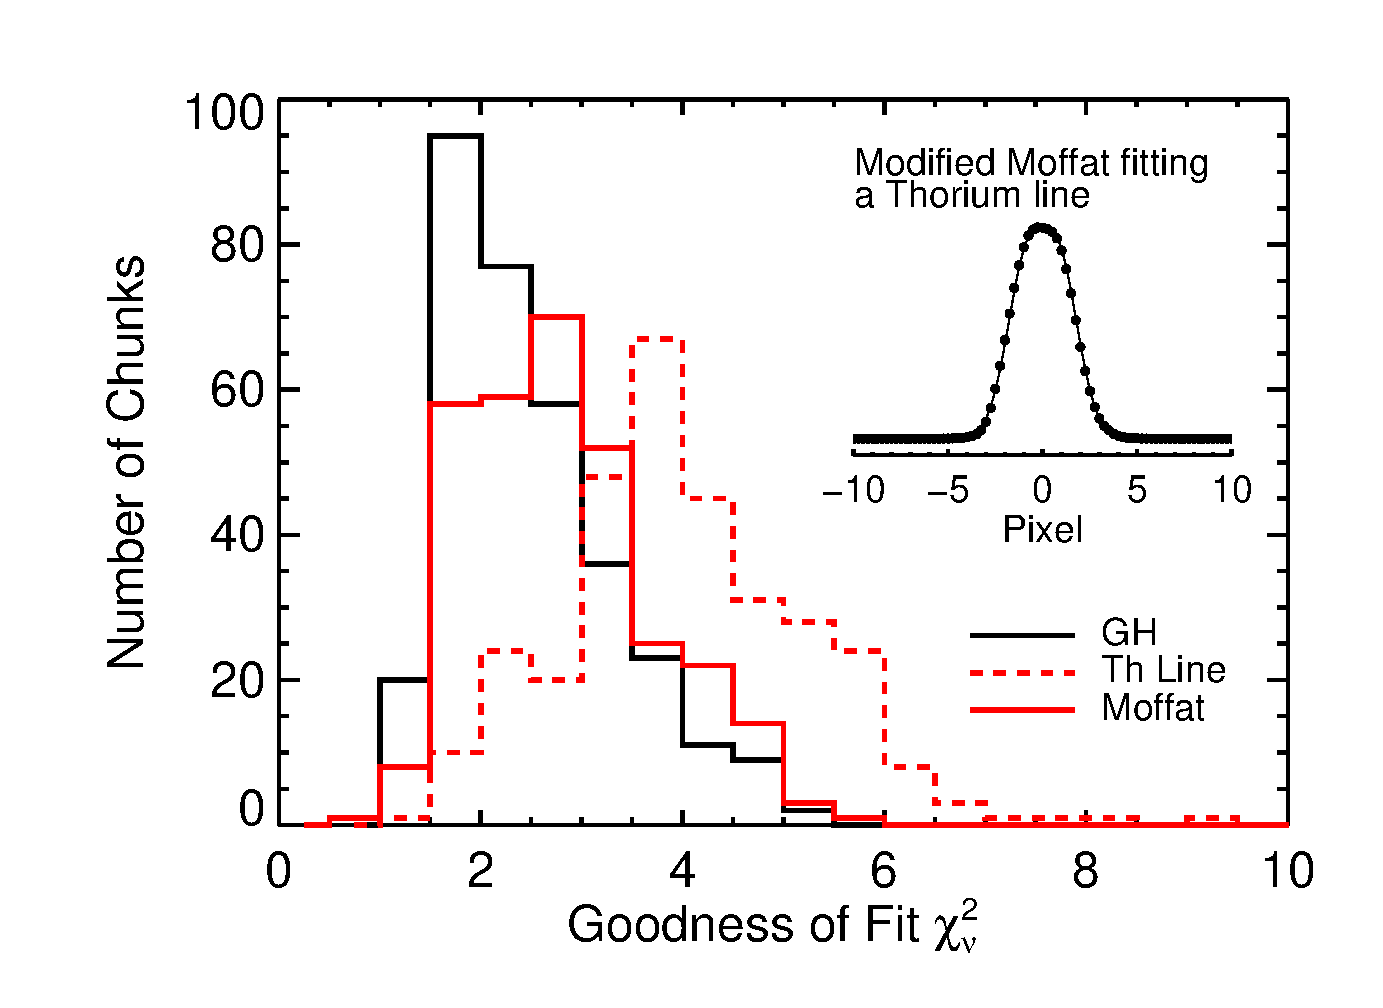
\includegraphics[scale=0.45]{het/thar_vs_moffat.eps}
\caption{Histogram of goodness of fit, $\chi^2_\nu$, values for
  spectral chunks of an iodine spectrum. The modified Moffat function
  (red) performs almost equally well while having only 3 parameters,
  com- pared with the complicated 11-parameter GH function (black
  solid). Red dashed histogram is for fits using a ThAr line profile
  as IP. The insert is showing the modified Moffat function can fit a
  ThAr line quite well.
\label{het:fig:moffat}}
\end{figure}
%----------------------------------------------------------------




